\section{Einleitung}

Der heutige Netzwerkverkehr ist fast tausendfach größer als vor 20 Jahre \citep{Roser_I}. Das Internet wird heutzutage für fast all unsere Tätigkeiten verwendet: Soziale Netzwerke, Video und Audio-Streaming, Einkauf, behördliche Angelegenheiten und viele andere. So viel Verkehr generiert eine unermessliche Menge von Daten, die alle möglichen Inhalte beinhalten, von unschuldigen Anfragen nach einem eigenen Kontostand bis zur Ausführung von beabsichtigten Anfragen, um Systeme lahmzulegen. Um ersteres vom letzterem zu unterscheiden, verwenden viele Firmen das sogenannte \glsfirst*{SIEM} oder Log-Analyse-Tools. 

Das \glsfirst{NIST} definiert \gls{SIEM} als Software für die Sammlung, Anpassung, Analyse, Überwachung und Bedrohungserkennung von Sicherheitsdaten aus verschiedenen Quellen \citep{NIST_Definitions}. Die Bewertung dieser Daten spielt eine wesentliche Rolle bei solchen Anwendungen, um zu entscheiden, ob es sich um legitime Anfrage oder um einen \glsplural{Cyberangriff} handelt. Mit den Daten von \gls{SIEM} kann das \glsfirst{SOC} Team Maßnahmen ergreifen. Log Analysis und Log Management beziehen sich auf die Sammlung, Bearbeitung, Speicherung und/oder Löschen, Weiterleitung und Überwachung von Loginformationen. In dieser Arbeit benutzen wir den Begriff \quotes{Log-Analyse-Tools}, um diese Systeme zu referenzieren.

In diesem Projekt recherchieren und vergleichen wir existierende \gls{SIEM} und Log-Analyse-Tools. Danach entscheiden wir uns für eine \gls{opensource} Lösung, um eine kostengünstige Verbreitung und Implementierung zu ermöglichen. Mit dem ausgewählten Tool analysieren und bewerten wir spezifische Logdateien, damit wir demnächst potenzielle Angriffe erkennen können. Die Regelsätzen für die Angriffserkennung sollen automatisch mithilfe der \glsfirst{ttp} von \gls{mitre} aufgebaut werden.

\newpage
Unser Ziel ist es, eine umfangreiche \gls{opensource} Lösung zu finden bzw. zu gesltaten, die uns ermöglicht, \glsplural{Cyberangriff} nach vordefinierten Regelsätzen zu detektieren. \glsplural{Proprietary} Lösungen gibt es viele auf dem Markt. Sie sind meistens kostenpflichtig und verlangen spezielle Wartung. Da sich solche Lösungen eher an große Konzerne richten, beschäftigen wir uns mit dem Aufbau und Strukturierung einer eigenen Lösung mithilfe von \gls{opensource} Tools. 

Diese Arbeit wird in folgende Teile geteilt: 

% OSSIN: https://sourceforge.net/projects/os-sim/
% Preludes: https://www.prelude-siem.org/projects/prelude/wiki/ManualUser
% ELK Stack

% Grafana / Promtail: https://grafana.com/products/enterprise/
%https://grafana.com/logs/% 

%https://www.ossec.net/         https://github.com/ossec/ossec-rules

% was machen sie konkrent? / Vergleich zwischen OpenSource/Proprietary/

{\setstretch{1.5}
\begin{itemize}[noitemsep]
   \item	Definition von SIEMs und Log-Analyse-Tools 
   \item	Beschreibung von existierenden \gls{Proprietary}en und Open Source Lösungen
   \item	Entscheidung für die Implementation einer Open Source Lösungen 
   \item	Installation und Konfiguration von der ausgewählten Anwendung 
   \item	Implementierung von zwei spezifischen Cyberangriffen 
   \item	Definition der \gls{usecases} und Implementierung von Regelsätze für die automatische Erkennung von der vorherigen Angriffen anhand der \gls{mitre} Matrix 
   \item	Empfang, Bearbeitung und Eingabe der spezifischen Logdateien der Hochschule in der ausgewählten Lösung  
\end{itemize}
}

\subsection{Problemstellung}
Während der Entwicklung dieser Arbeit beschäftigen wir uns mit folgenden Fragenstellung: 

{\setstretch{1.5}
% Regeln anhand mittre, automatisieren
\begin{itemize}[noitemsep]
   \item Wie können wir ein Log-Analyse-Tool konfigurieren, dass es vordefinierte Angriffe nach der \gls{mitre} Matrix automatisch erkennen kann? 
   \item Wie können wir allgemeine \glsplural{usecases} definieren, sodass wir sie später für verschiedene Angriffsmuster nach \gls{mitre} Matrix leicht anpassen können?
\end{itemize}
}

% \newpage
% \subsection{Vorgehensweise}
% Um diese oben genannten Ziele zu erreichen, verwenden wir folgenden Methoden: 

% {\setstretch{1.5}
% \begin{itemize}[noitemsep]
%    \item	Recherche in der Fachliteratur über SIEMs und Log-Analyse-Tools Lösungen 
%    \item	Vergleich zwischen verschiedenen Open Source und \gls{Proprietary}en Lösungen 
%    \item	Installation von dem ausgewählten Tool 
%    \item	Importieren von Logdateien in der ausgewählten Lösung 
%    \item	Definition der Use Cases für die Angriffe
% \end{itemize}
% }

\newpage
Das folgende Diagramm, \ref{fig:AblaufderArbeit}, stellt den Aufbau und Entwicklung dieser Arbeit dar, wie oben beschrieben:
% Diagram anpassen mit korrenkten Zielen

\begin{figure}[H]
   \centering
   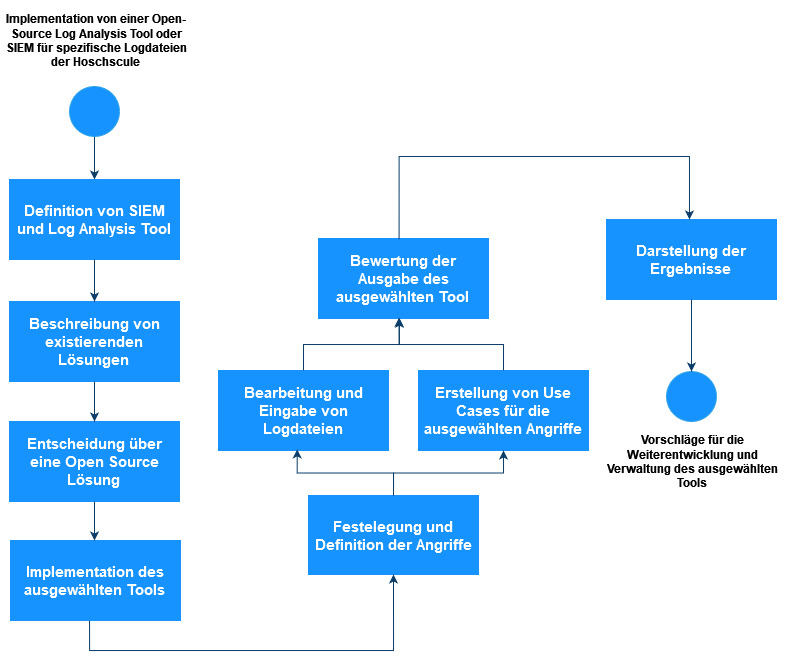
\includegraphics[width=1\textwidth]{assets/1_p1.jpg}
   \caption[Aufbau dieser wissenschaftlichen Recherche]
   {Aufbau dieser wissenschaftlichen Recherche \\Quelle: Eigene Darstellung }
   \label{fig:AblaufderArbeit}
   \centering
\end{figure}



